\documentclass[12pt,a4paper,titlepage]{article}
\usepackage{lab_style}
\usepackage{pdfpages}
\usepackage{eso-pic}
\usepackage{graphicx}
\usepackage{float}
\newcommand\tab[1][1cm]{\hspace*{#1}}

\graphicspath{ {./} }
  
\begin{document}

\begin{titlepage}
\selectlanguage{english}

%----------------------------------------------------------------------------------------
% TITLE PAGE INFORMATION
%----------------------------------------------------------------------------------------
  \begin{center} % Center everything on the page

  %----------------------------------------------------------------------------------------
  % HEADING SECTIONS
  %----------------------------------------------------------------------------------------
  \textsc{\large Faculty of Computers, Informatics and Microelectronics}\\[0.5cm]
  \textsc{\large Technical University of Moldova}\\[1.2cm] % Name of your university/college
  \vspace{25 mm}

  \textsc{\Large Object-Oriented Modeling and Analysis}\\[0.5cm] % Major heading such as course name
  \textsc{\large Laboratory work \#7}\\[0.5cm] % Minor heading such as course title

\newcommand{\HRule}{\rule{\linewidth}{0.5mm}} % Defines a new command for the horizontal lines, change thickness here

  %----------------------------------------------------------------------------------------
  % TITLE SECTION
  %----------------------------------------------------------------------------------------
  \vspace{10 mm}
  \HRule \\[0.4cm]
  { \LARGE \bfseries Modeling your project with Activity Diagrams. Application delivery. Software life-cycle. }\\[0.4cm] % Title of your document
  \HRule \\[1.5cm]

  %----------------------------------------------------------------------------------------
  % AUTHOR SECTION
  %----------------------------------------------------------------------------------------
      \vspace{30mm}

      \begin{minipage}{0.4\textwidth}
      \begin{flushleft} \large
      \emph{Author:}\\
      Cernei \textsc{Liviu}
      \end{flushleft}
      \end{minipage}
      ~
      \begin{minipage}{0.4\textwidth}
      \begin{flushright} \large
      \emph{Supervisor:} \\
      Mihail \textsc{Gavrilița} % Supervisor's Name
      \end{flushright}
      \end{minipage}\\[4cm]

      \vspace{5 mm}
      % If you don't want a supervisor, uncomment the two lines below and remove the section above
      %\Large \emph{Author:}\\
      %John \textsc{Smith}\\[3cm] % Your name

      %----------------------------------------------------------------------------------------
      % DATE SECTION
      %----------------------------------------------------------------------------------------

      {\large Chișinau 2018}\\[3cm] % Date, change the \today to a set date if you want to be precise

      %----------------------------------------------------------------------------------------
      % LOGO SECTION
      %----------------------------------------------------------------------------------------

      %\includegraphics{red}\\[0.5cm] % Include a department/university logo - this will require the graphicx package

      %----------------------------------------------------------------------------------------

      \vfill % Fill the rest of the page with whitespace
      \end{center}
      
\end{titlepage}

\cleardoublepage

\newpage

\pagenumbering{arabic}
\setcounter{page}{1}
\setcounter{secnumdepth}{4}

\addtocontents{toc}{\protect\thispagestyle{empty}} % no page number on the table of contents page
\cleardoublepage


\phantomsection
\addcontentsline{toc}{section}{Introduction}
\section*{Laboratory work \#7}
\phantomsection

\section{Tasks}
\begin{itemize}
	\item
	Model your application using 3 Activity Diagrams;
	\item 
	Document the Application Delivery / Installation.
\end{itemize}

\section{Theory}

\subsection{Software Development Process}
In software engineering, a software development process is the process of dividing software development work into distinct phases to improve design, product management, and project management. It is also known as a software development life cycle. The methodology may include the pre-definition of specific deliverables and artifacts that are created and completed by a project team to develop or maintain an application.\par
Most modern development processes can be vaguely described as agile. Other methodologies include waterfall, prototyping, iterative and incremental development, spiral development, rapid application development, and extreme programming.\par
Some people consider a life-cycle "model" a more general term for a category of methodologies and a software development "process" a more specific term to refer to a specific process chosen by a specific organization. For example, there are many specific software development processes that fit the spiral life-cycle model. The field is often considered a subset of the systems development life cycle.\par
\clearpage

\section{Activity Diagrams}
In Figure ~\ref{fig:login} is represented the activity diagram for user login.
\begin{figure}[H]
\centering
	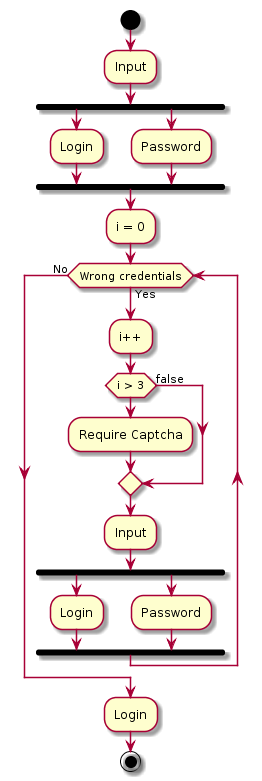
\includegraphics[width=5cm]{login}
	\caption{Login activity diagram}
	\label{fig:login}
\end{figure}
To login in an account, the user inputs login and password in any order. Then the input is submitted. If the credentials are right, the user is authenticated successfully. Otherwise, it should try again. If the third attempt is unsuccessful, he is requested to pass the captcha test. Any attempt from that moment will requre the additional test, until he inputs correct data.


\section{Application Delivery / Installation}
The last step of website development is deployment. The process of“getting your website on the web” consists of a number of steps:

\begin{itemize}
	\item
	Finding a domain name
\item
	Finding a hosting service
\item
	Uploading files with SFTP
	\item 
	Deploying server-side applications
\end{itemize}

But the client is not required to download or install anything. He simply navigates to the webpage. The only step he should take is to create an account.

\section{Conclusion}
In this laboratory work we learned to create activity diagrams and explain Application Delivery / Installation.

\clearpage
\cleardoublepage

\end{document}
